%
% File: chap06.tex
% Author: Nadeem Gul Rintu Daniel
% Description: Goes through the development environment for Android and the setup procedure.
%
\let\textcircled=\pgftextcircled
\chapter{Implementation Consideration}
\label{chap:implementationConsideration}
\noindent
\initial{T}his section gives an overview of the Development tools used for the implementation of the Floe Navigation System. It will briefly introduce the software development tools used to create the App. It also gives a detailed description of the setup procedure of the development environment in which the Floe Navigation System was implemented. 
%
%
\section{Development Environment}
\label{sec:sec6_1}
\noindent
%
The Floe Navigation System consists of the Floe Navigation App and the Synchronization Server; each of which is developed in a separate environment. The Floe Navigation App is developed in Android and the Synchronization Server consists of a MySQL Database and PHP based Web-services.
Table~\ref{tbl:CH6applicationsUsed} shows the layers that are visible on the Grid by default along with their respective icons.
%
\begin{table}[!htbp]
	\centering
	\begin{tabular}{ |m{7.5cm}| m{2.5cm} | }
		\hline
		\textbf{Application}  &  \textbf{Version}\footnotemark[1]  \\
		\hline
		Java JRE&1.8.0\textunderscore52
		\\ \hline
		Android Studio&3.2.1
		\\ \hline
		Eclipse IDE\footnotemark[2]&Neon.3 Release (4.6.3)
		\\ \hline
		MySQL\footnotemark[2]&8.0
		\\ \hline
		Postman\footnotemark[2]&6.6.0 
		\\ \hline
		Microsoft Internet Information Services\footnotemark[2]&10.0.17134.1
		\\ \hline
		
	\end{tabular}
	\mycaption[Applications Used in System Development.]{Applications Used in System Development.}
	\label{tbl:CH6applicationsUsed}
\end{table}
\footnotetext[1]{Versions used for developing Floe Navigation App version 1.0.0.}
\footnotetext[2]{Used only for Synchronization. For changes in the App which do not affect the Synchronization process, you will only need Android Studio.}
%
\subsection{Setting Up Android Development Environment}
\label{sec:sec6_1_1}
\noindent
The Floe Navigation App was developed using Android Studio. Android Studio is the official Integrated Development Environment (IDE) for development of Android Apps. Android Studio is connected to the tablet using Android Debug Bridge (ADB). The Android Debug Bridge is a software-interface for the Android system, which can be used to connect an android device with a computer using a USB cable or a wireless connection~\cite{droidwiki}.
\newline
\noindent
However, the tablet used in this system (XSLATE D$10$) does not support a USB Slave connection~\cite{tablet:xslated10} for debugging and through testing it was observed that the WiFi Access Point of the AIS Transponder em-trak B$360$ does not support more than one client simultaneously. In addition to the Wifi and the USB interfaces, the tablet also has an Ethernet interface~\cite{tablet:xslated10}, however, Android does not support multiple network interfaces simultaneously so when connecting with ADB over Ethernet the tablet will not be able to connect to the WiFi network of the AIS Transponder. So Bluetooth tethering was used to connect the tablet with the PC over ADB for code debugging and flashing and the Wifi interface was available for connection with the AIS transponder.
\newline
\noindent
Follow the steps below to setup ADB over Bluetooth:
\begin{enumerate}
	\item Enable Developer Options and Android Debugging on the tablet by going to Settings $\to$ System $\to$ About Phone and tap the Build Number $7$ times.
%
	\item Connect the PC to the tablet via Ethernet and assign Static IPs to both the tablet and the PC. Static IP Assignment on the tablet XSLATE D$10$ is shown in figure~\ref{fig:CH6staticIPAssign}
		\begin{figure}[h]
			\centering
			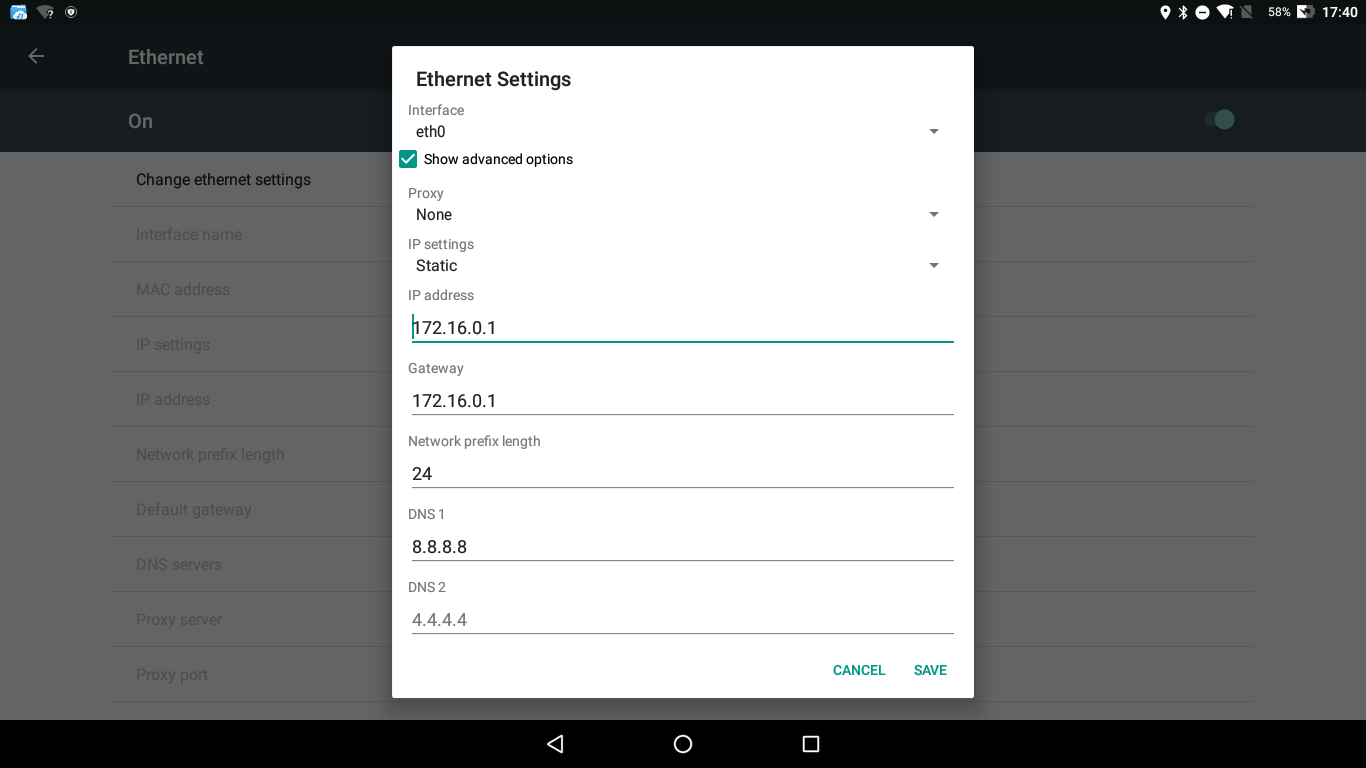
\includegraphics[height=0.3\textheight]{fig06/staticIpAssignTab.png}
			\mycaption[Assigning Static IP to Ethernet Connection on the Tablet.]{Assigning Static IP to Ethernet Connection on the Tablet. }
			\label{fig:CH6staticIPAssign}
		\end{figure}
%
	\item Open a Command Prompt window on the PC and start Android Debugging Bridge (ADB) in TCP IP mode by entering the following commands (Enter the IP of the tablet):
		\begin{lstlisting}[style=DOS]
			>adb connect ***.***.***.***
			>adb tcpip 4455
		\end{lstlisting}
%
	\item Enable Bluetooth on the tablet and pair the tablet with the PC.
%
	\item On the tablet go to Settings$\to$More$\to$Tethering \& portable hotspot and enable Bluetooth tethering as shown in figure~\ref{fig:CH6enableBluetoothTethering}.
		\begin{figure}[h]
			\centering
			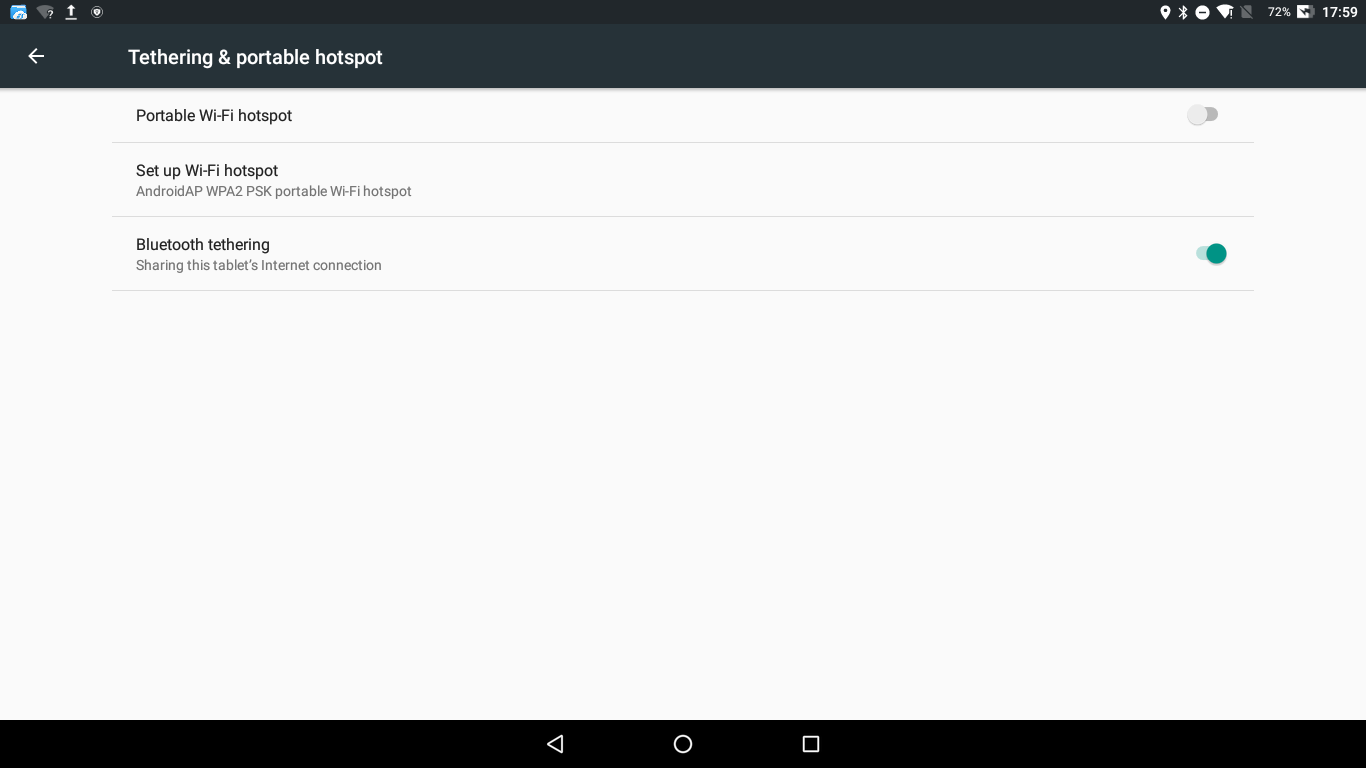
\includegraphics[height=0.3\textheight]{fig06/BluetoothTetheringEnable.png}
			\mycaption[Enabling Bluetooth Tethering on tablet.]{Enabling Bluetooth Tethering on tablet.}
			\label{fig:CH6enableBluetoothTethering}
		\end{figure}
%
	\item On the PC go to Control Panel$\to$Devices and Printers and right-click on the tablet and click on Connect Using$\to$Access Point as shown in figure~\ref{fig:CH6connectAccessPoint}. 
		\begin{figure}[h]
			\centering
			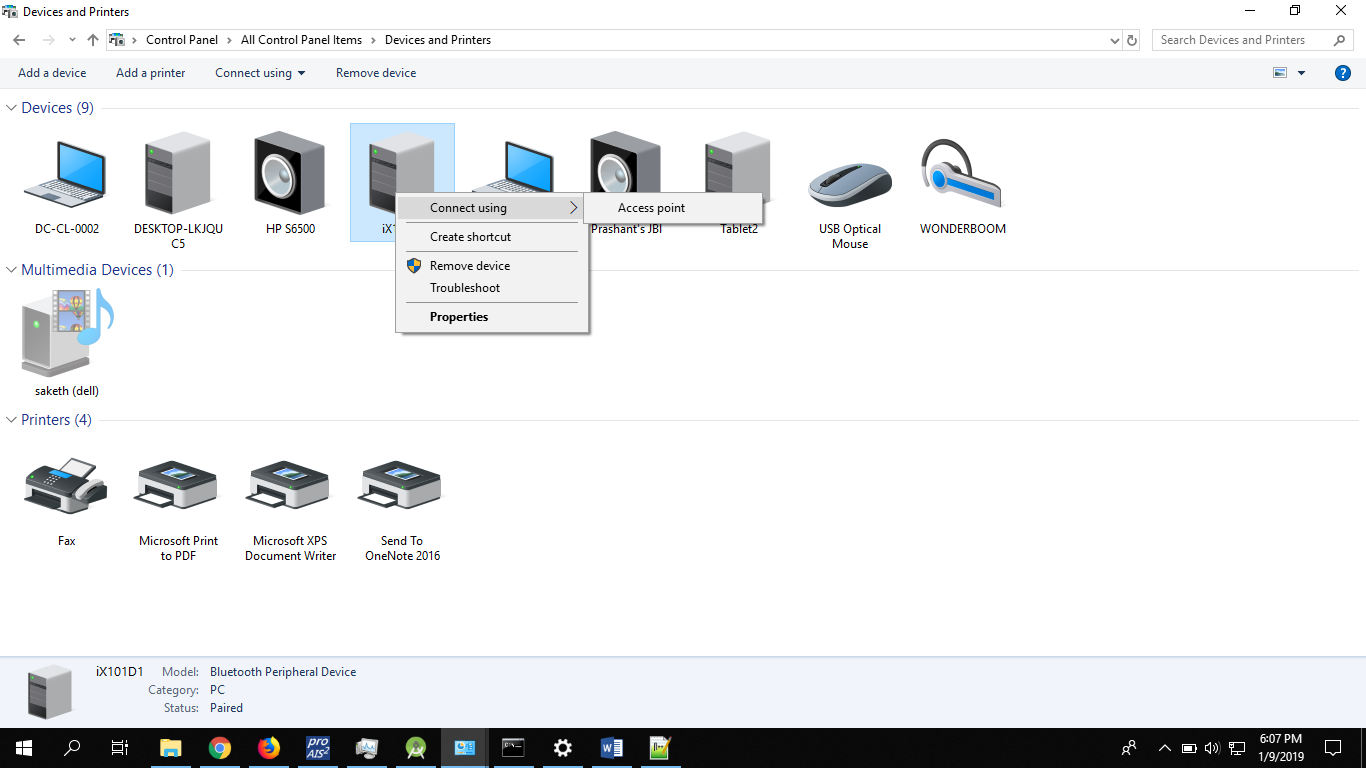
\includegraphics[height=0.3\textheight]{fig06/connectAccessPoint.png}
			\mycaption[Connect to Bluetooth Access Point.]{Connect to Bluetooth Access Point.\textbf{\textcolor{red}{Insert better screenshot}}}
			\label{fig:CH6connectAccessPoint}
		\end{figure}
\newline
\noindent
If on right-clicking the tablet and Connect Using shows Direct Connection instead of Access Point try unpairing and repairing the tablet with the PC.
%
	\item Now go back to the command prompt and enter:
		\begin{lstlisting}[style=DOS]
			>adb connect 192.168.44.1:4455
		\end{lstlisting} 	
\end{enumerate}
The PC is now connected to the tablet and you can deploy your App to the tablet and/or debug it as can be seen from figure~\ref{fig:CH6DeploymentOverBluetooth}.
\begin{figure}[h]
	\centering
	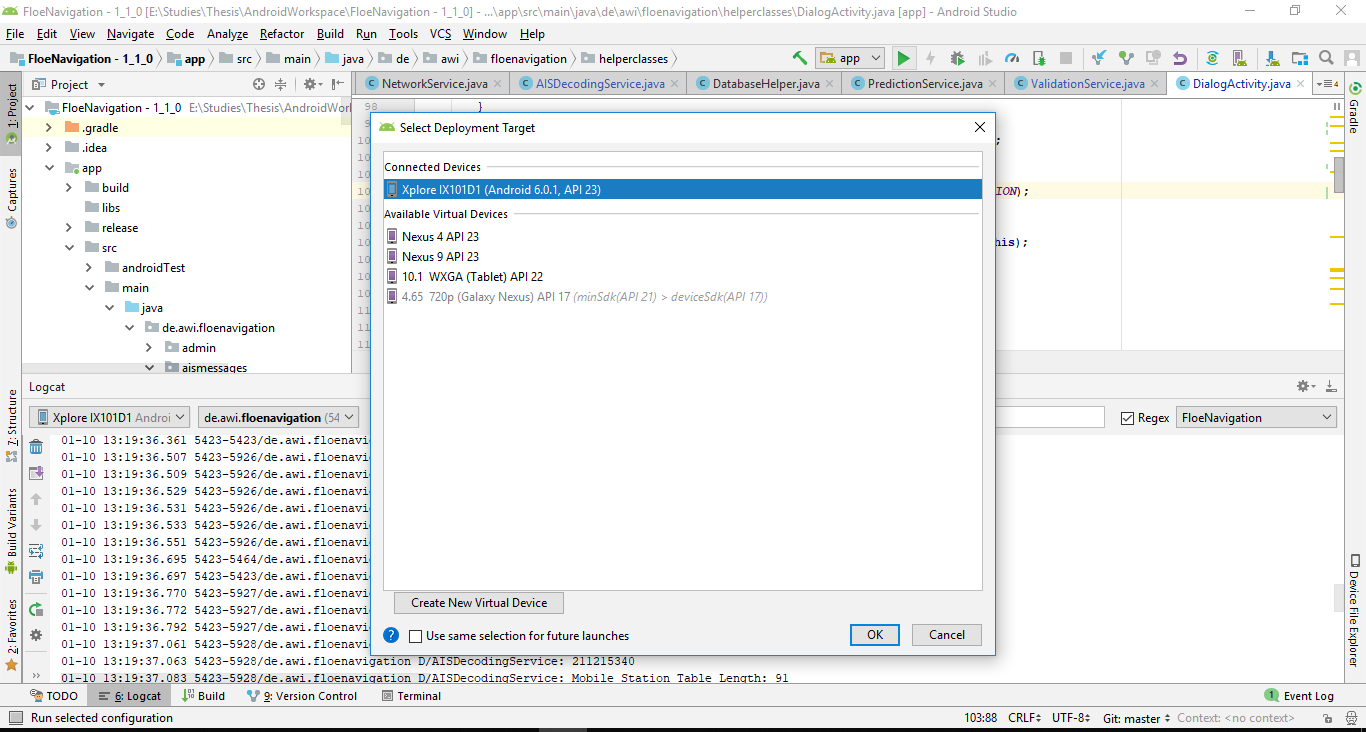
\includegraphics[height=0.3\textheight]{fig06/DeploymentOverBluetooth.png}
	\mycaption[App Deployment from Android Studio using ADB over Bluetooth.]{App Deployment from Android Studio using ADB over Bluetooth. \textbf{\textcolor{red}{Insert better screenshot}}}
	\label{fig:CH6DeploymentOverBluetooth}
\end{figure}
\newline
\noindent
The logs from the tablet can also be viewed using the Logcat window in Android Studio as can be seen from figure~\ref{fig:CH6LogcatOverBluetooth}.
\begin{figure}[h]
	\centering
	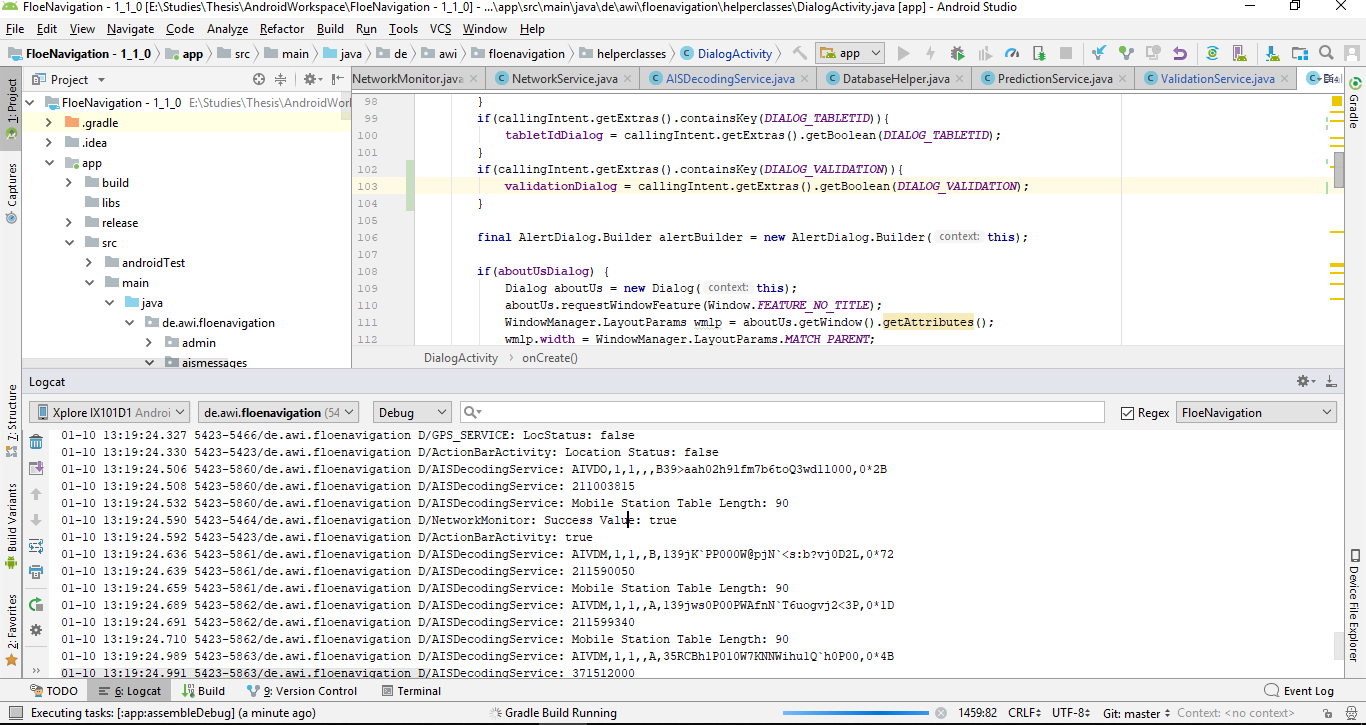
\includegraphics[height=0.3\textheight]{fig06/logcatOverBluetooth.png}
	\mycaption[Logcat Window in Android Studio displaying the Logs from the tablet.]{Logcat Window in Android Studio displaying the Logs from the tablet. \textbf{\textcolor{red}{Insert better screenshot}}}
	\label{fig:CH6LogcatOverBluetooth}
\end{figure}  